\sectionnewpage
\section{Slope fields}
\label{slopefields:section}

\LAtt{1.2}

\LO{
\item Identify or sketch a slope field for a first order differential equation and
\item Use the slope field to determine the trajectory of a solution to a differential equation. 
}

% \sectionnotes{0.5 lecture\EPref{, \S1.3 in \cite{EP}}\BDref{,
% \S1.1 in \cite{BD}}}

%At this point it may be good to first try the
%Lab I\index{IODE software!Lab I} and/or Project I\index{IODE software!Project I} from the
%IODE website: \url{http://www.math.uiuc.edu/iode/}.
%
%\medskip

As we said, the general first order equation we are studying looks like
\begin{equation*}
y' = f(x,y).
\end{equation*}
A lot of the time, we cannot simply solve these kinds of equations explicitly, because our direct integration method only works when the equation is of the form $y' = f(x),$ which we could integrate directly. In these more complicated cases, it would be nice if we could at least figure out the shape and behavior of
the solutions, or find approximate solutions.

\subsection{Slope fields}

%As you have seen in IODE Lab I (if you did it),
\begin{mywrapfig}{2.75in}
\capstart
\diffyincludegraphics{width=2.5in}{width=4in}{1-3-xysl-one}
\caption{The slope $y'=xy$ at $(2,1.5)$.\label{1.3:fig0}}
\end{mywrapfig}

Suppose that we have a solution to the equation $y' = f(x,y)$ with $y(x_0) = y_0$. 
What does the fact that this solves the differential equation tell us about the solution?
 It tells us that the derivative of the solution at this point will be 
$f(x_0, y_0)$. Graphically, the derivative gives the slope of the solution,
 so it means that the solution will pass through the point $(x_0, y_0)$ and will have slope $f(x_0, y_0)$. 
For example, if $f(x,y) = xy$, then at point $(2,1.5)$ we draw a
short line of slope $xy = 2 \times 1.5 = 3$.  So, if $y(x)$ is a solution
and $y(2) = 1.5$, then the equation mandates that $y'(2) = 3$.
See \figurevref{1.3:fig0}.

To get an idea of how solutions behave, we draw such lines at lots
of points in the plane, not just the point $(2,1.5)$.  We would
ideally want to see the slope at every point, but that is
just not possible.  Usually we pick a
grid of points fine enough so that it shows the behavior, but not too
fine so that we can still recognize the individual lines.
We call this picture the \emph{\myindex{slope field}} of the equation.
See \figurevref{1.3:fig1} for the slope field of the equation $y' = xy$.
Usually in practice, one does not do this by hand, but has a computer do the
drawing.

The idea of a slope field is that it tells us how the graph of the solution should be sloped, 
or should curve, if it passed through a given point. Having a wide variety of slopes 
plotted in our slope field gives an idea of how all of the solutions behave for a bunch of different 
initial conditions. Which curve we want in particular, and where we should start the curve, depends on the initial condition. 

Suppose we are given a specific initial condition $y(x_0) = y_0$.
A solution, that is, the graph of the solution, would be a curve
that follows the slopes we drew, starting from the point $(x_0, y_0)$. 
For a few sample
solutions, see \figurevref{1.3:fig2}.  It is easy to roughly sketch
(or at least imagine)
possible solutions in the slope field, just from looking at the slope field
itself.  You simply sketch a line that roughly fits the little line segments
and goes through your initial condition. The graph should ``flow'' along the little slopes that are on the slope field. 

\begin{myfig}
\parbox[t]{2.5in}{\capstart%
 \diffyincludegraphics{width=2.5in}{width=4.5in}{1-3-xysl}
 \caption{Slope field of $y' = xy$.\label{1.3:fig1}} 
 }
\quad \qquad
\parbox[t]{2.5in}{ \capstart
 \diffyincludegraphics{width=2.5in}{width=4.5in}{1-3-xysl-sol}
 \caption{Slope field of $y' = xy$ with a graph of solutions satisfying
 $y(0) = 0.2$, $y(0) = 0$, and $y(0) = -0.2$.\label{1.3:fig2}}
}
\end{myfig}

By looking at the slope field we get a lot of information
about the behavior of solutions without having to solve
the equation.  For
example, in \figurevref{1.3:fig2} we see what the solutions do when the initial conditions
are $y(0) > 0$, $y(0) = 0$ and $y(0) < 0$.
A small change in the
initial condition causes quite different behavior.
We see this behavior just
from the slope field and imagining what solutions ought to do.

We see a different behavior for the equation
$y' = -y$.  The slope field and a few solutions is in
see \figurevref{1.3:fig3}.
If we think of moving from left to right (perhaps $x$ is time
and time is usually increasing), then
we see that no matter what $y(0)$ is, all solutions tend to zero as $x$
tends to infinity.
Again that behavior is clear from simply
looking at the slope field itself.

\begin{myfig}
\capstart
\diffyincludegraphics{width=2.5in}{width=4in}{1-3-mysl-sol}
\caption{Slope field of $y' = -y$ with a graph of a few solutions.\label{1.3:fig3}}
\end{myfig}

\subsection{Exercises}

\begin{exercise}
Sketch slope field for $y'=e^{x-y}$.  How do the solutions behave as $x$
grows?  Can you guess a particular solution by looking at the slope
field?
\end{exercise}
\comboSol{%
}
{%
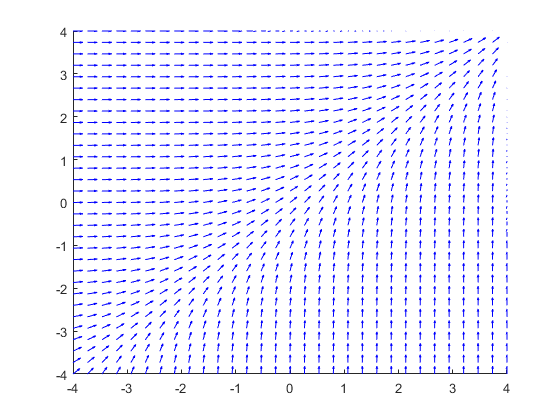
\includegraphics[width=2in]{Images/slopefieldexpxmy.png}

$y=x$ is a solution.
}

\begin{exercise}\ansMark%
Sketch the slope field of $y'=y^3$.  Can you visually find the solution
that satisfies $y(0)=0$?
\end{exercise}
\exsol{%
\\[6pt]
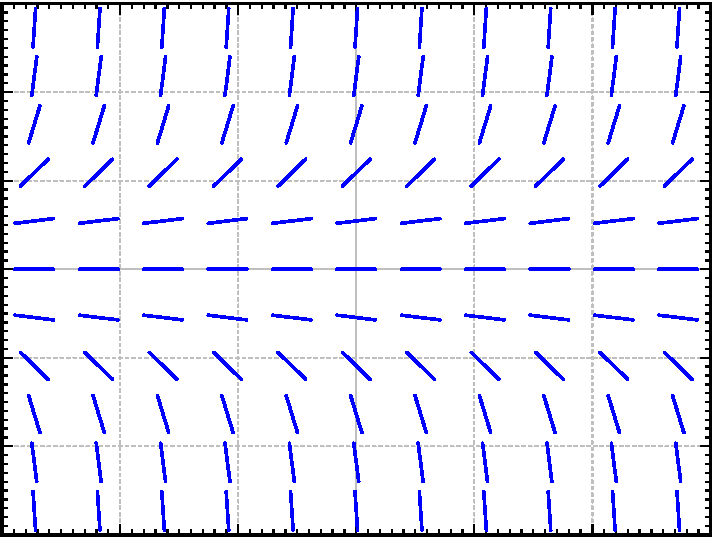
\includegraphics[width=2in]{figures/yprimey3slope}
\\
$y=0$ is a solution such that $y(0)=0$.
}


\begin{exercise}
Sketch slope field for $y'=x^2$.
\end{exercise}
\comboSol{%
}
{%
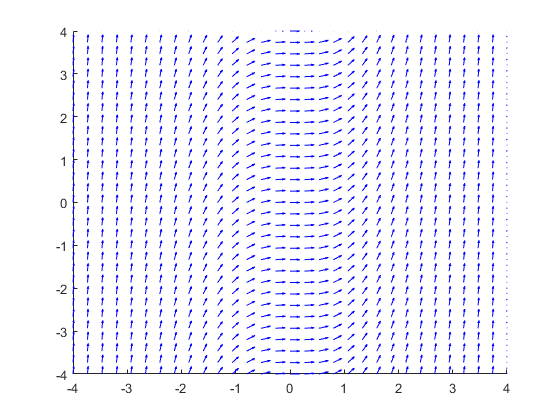
\includegraphics[width=2in]{Images/slopefieldx2.png}
}

\begin{exercise}
Sketch slope field for $y'=y^2$.
\end{exercise}
\comboSol{%
}
{%
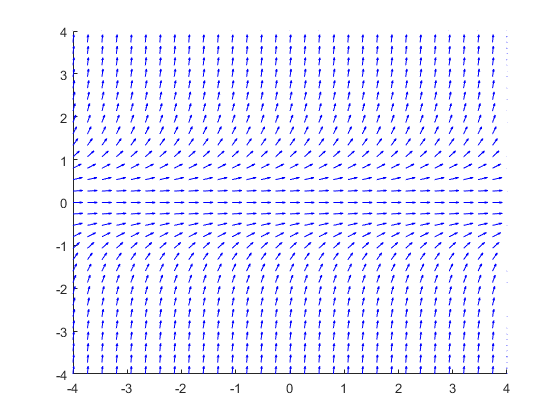
\includegraphics[width=2in]{Images/slopefieldy2.png}
}

\begin{exercise}
For each of the following differential equations, sketch out a slope field on $-3 < x < 3$ and $-3 < y < 3$ and determine the overall behavior of the solutions to the equation as $t \rightarrow \infty$. If this fact depends on the value of the solution at $t=0$, explain how it changes.
\begin{tasks}(4)
\task $\displaystyle \frac{dy}{dx} = 3 - 2y$
\task $\displaystyle \frac{dy}{dx} = 1 + y$
\task $\displaystyle \frac{dy}{dx} = y - 1$
\task $\displaystyle \frac{dy}{dx} = -2 - y$
\end{tasks}
\end{exercise}
\comboSol{%
}
{%
a)~\parbox[c]{1.2in}{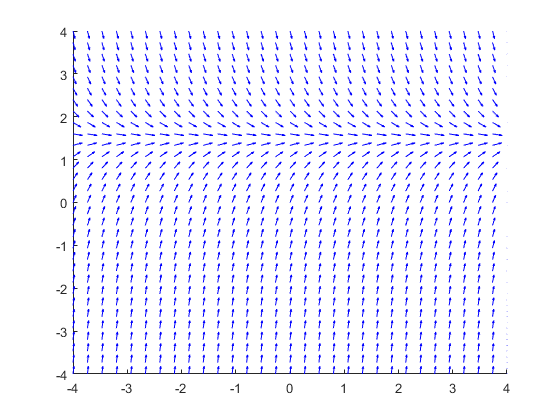
\includegraphics[width=1.2in]{Images/slopefield3m2y.png}} \quad b)~\parbox[c]{1.2in}{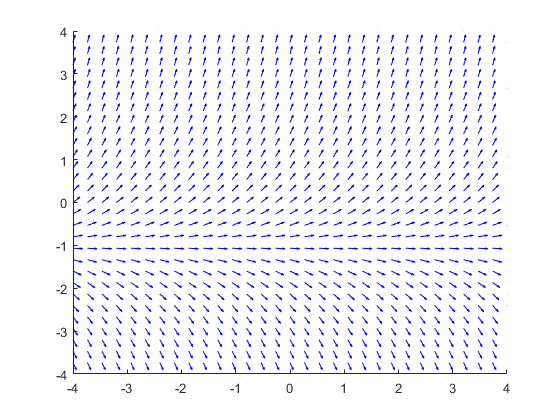
\includegraphics[width=1.2in]{Images/slopefield1py.png}} \quad c)~\parbox[c]{1.2in}{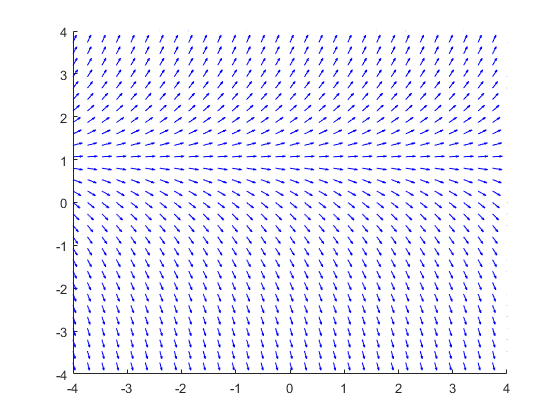
\includegraphics[width=1.2in]{Images/slopefieldym1.png}} \quad d)~\parbox[c]{1.2in}{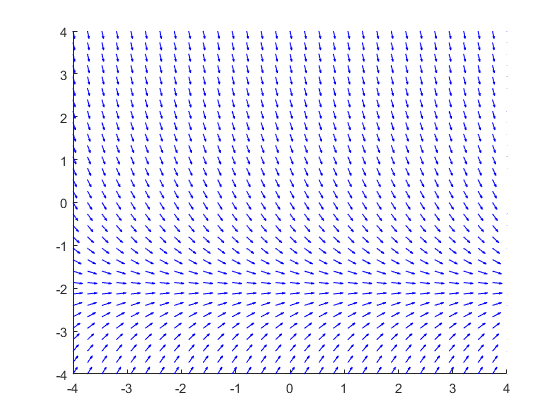
\includegraphics[width=1.2in]{Images/slopefieldm2my.png}}

a)~Solutions tend to $3/2$.
b)~Solutions go to $\infty$ if $y(0) > -1$, goes to $-\infty$ is $y(0) < -1$. Constant if $y(0) = -1$. 
c)~Solutions go to $\infty$ if $y(0) > 1$, goes to $-\infty$ is $y(0) < 1$. Constant if $y(0) = 1$. 
d)~Solutions tend to $-2$.
}

\begin{exercise}
Which of the following slope fields corresponds to the differential equation $\frac{dy}{dt} = t(y-1)$. Explain your reasoning.
\begin{tasks}(3)
\task
\parbox[c]{1.75in}{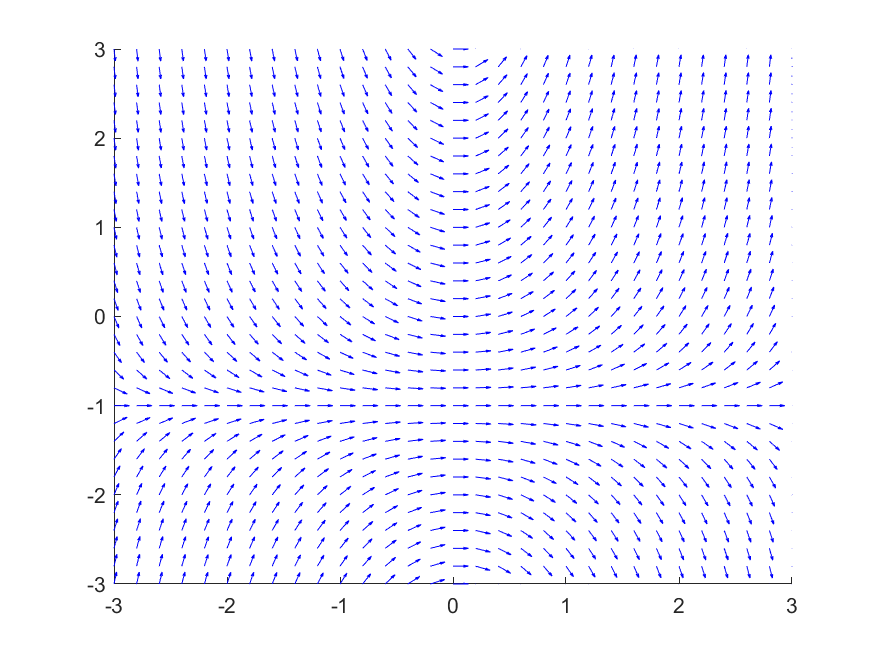
\includegraphics[width=1.75in]{Images/yprimetyp1slope}}
\task
\parbox[c]{1.75in}{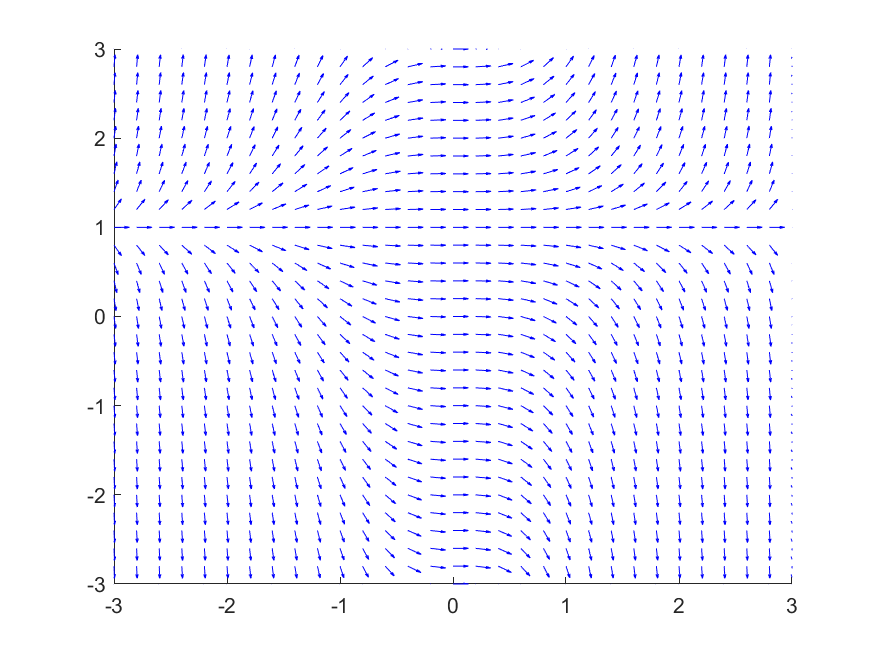
\includegraphics[width=1.75in]{Images/yprimetsqym1slope}}
\task
\parbox[c]{1.75in}{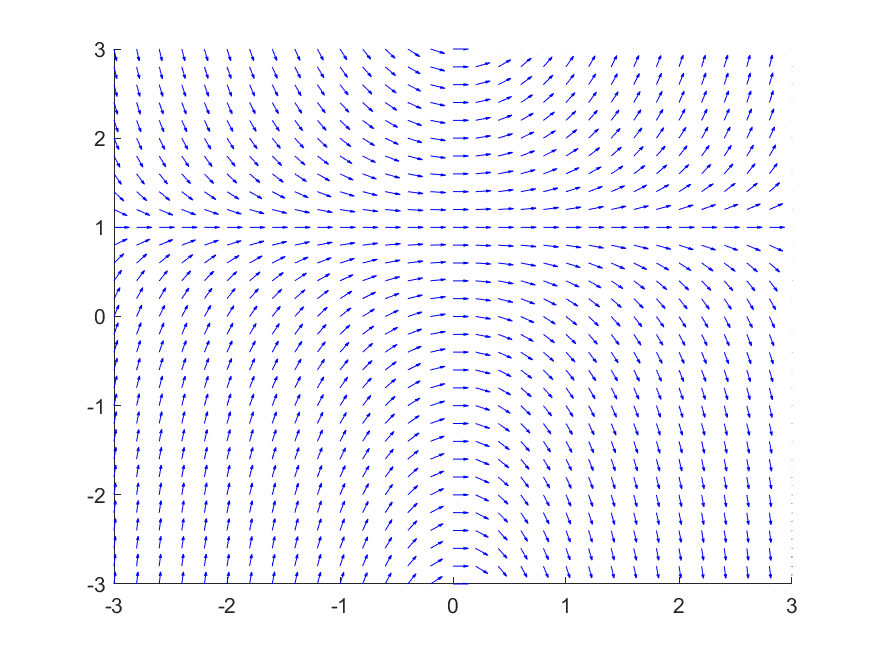
\includegraphics[width=1.75in]{Images/yprimetym1slope}}
\end{tasks}
\end{exercise}
\comboSol{%
}
{%
c)
}

\begin{exercise}
Which of the following slope fields corresponds to the differential equation $\frac{dy}{dt} = (2-t)(y^2 - 9)$. Explain your reasoning.
\begin{tasks}(3)
\task
\parbox[c]{1.75in}{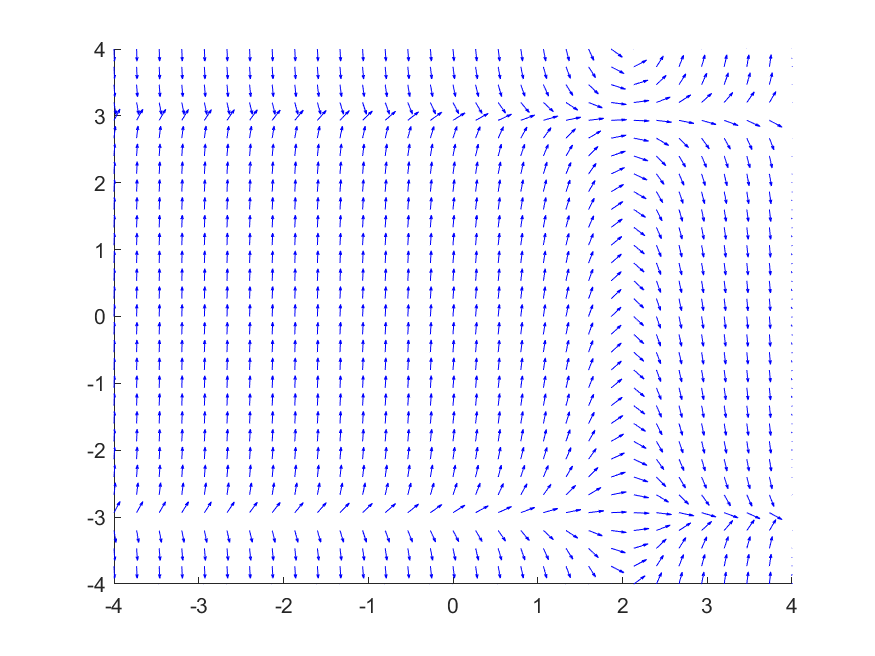
\includegraphics[width=1.75in]{Images/yprimetm2ysqm9slope}}
\task
\parbox[c]{1.75in}{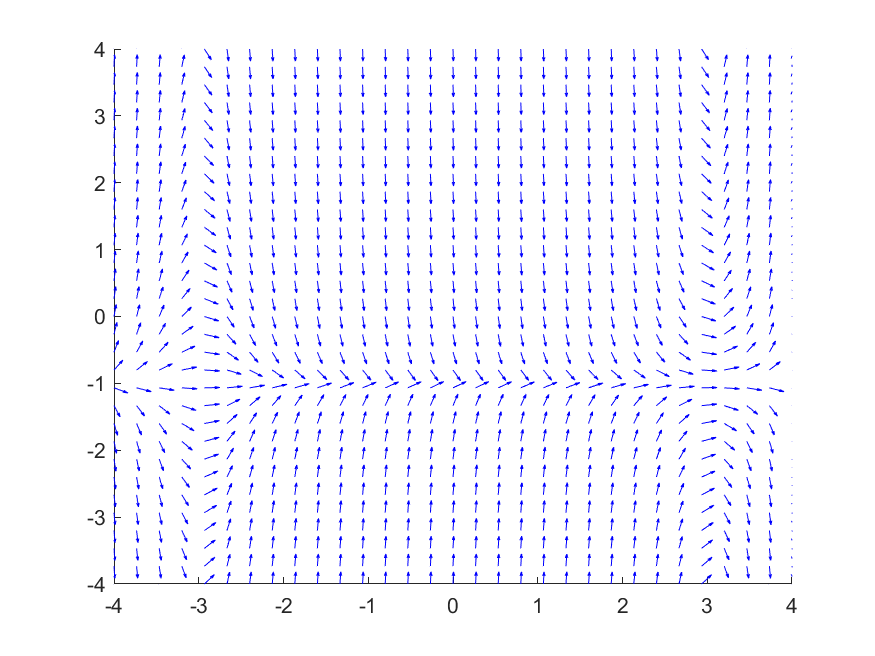
\includegraphics[width=1.75in]{Images/yprimeyp1tsqm9slope}}
\task
\parbox[c]{1.75in}{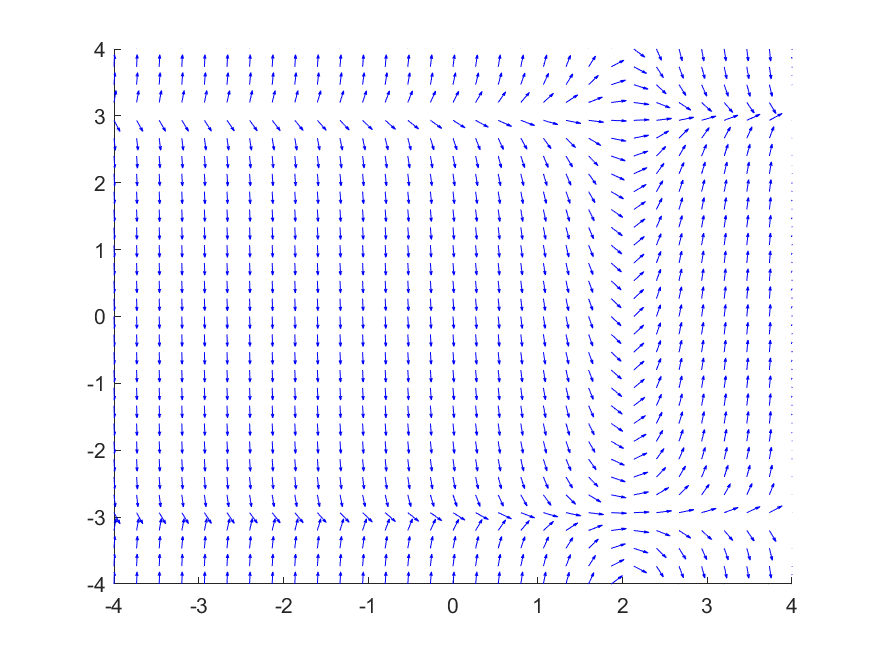
\includegraphics[width=1.75in]{Images/yprime2mtysqm9slope}}
\end{tasks}
\end{exercise}
\comboSol{%
}
{%
a)
}


\newpage

\begin{exercise}
Match equations $y'=1-x$, $y'=x-2y$, $y' = x(1-y)$ to slope fields.
Justify.
\begin{tasks}(3)
\task
\parbox[c]{1.75in}{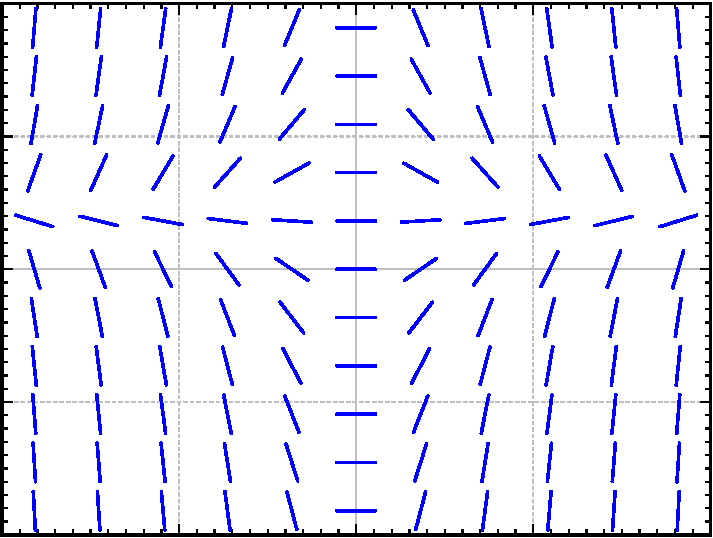
\includegraphics[width=1.75in]{figures/yprimex1minusyslope}}
\task
\parbox[c]{1.75in}{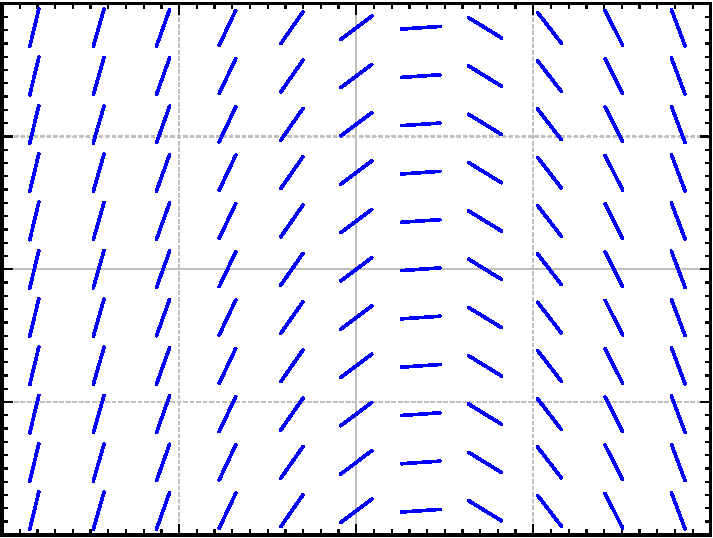
\includegraphics[width=1.75in]{figures/yprime1minusxslope}}
\task
\parbox[c]{1.75in}{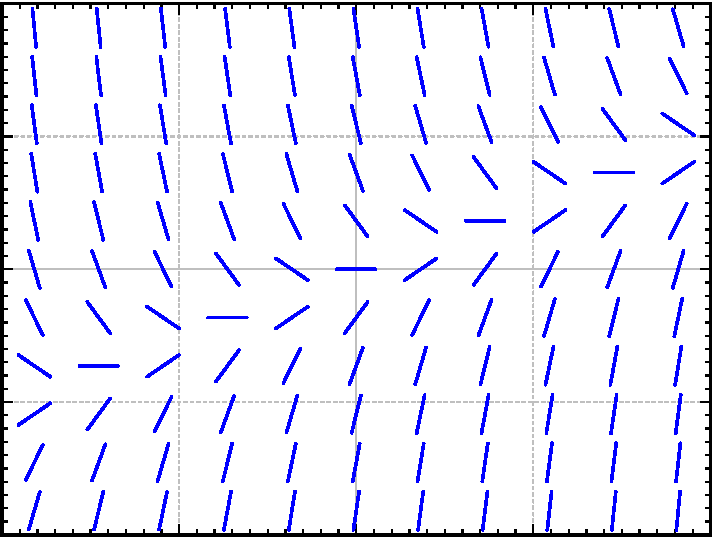
\includegraphics[width=1.75in]{figures/yprimexminus2yslope}}
\end{tasks}
\end{exercise}
\comboSol{%
}
{%
a)~$y' = x(1-y)$ \quad b)~$y' = 1-x$ \quad c)~$y'=x-2y$
}


\begin{exercise}\ansMark%
Match equations $y'=\sin x$, $y'=\cos y$, $y' = y\cos(x)$ to slope fields.
Justify.
\begin{tasks}(3)
\task
\parbox[c]{1.75in}{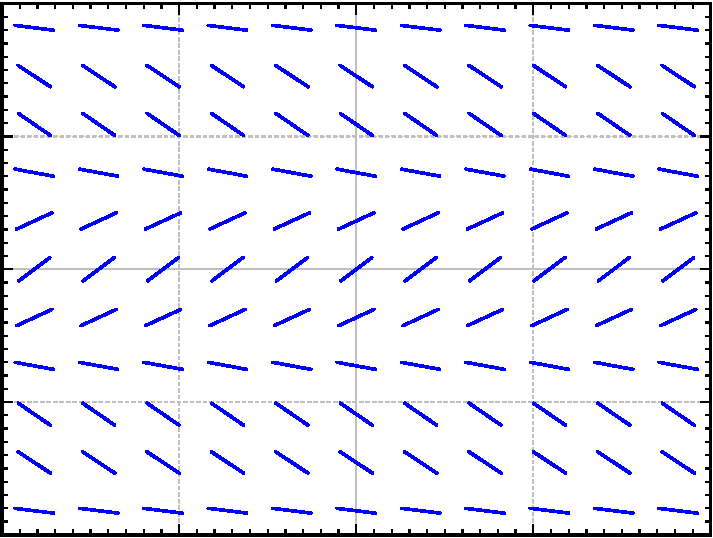
\includegraphics[width=1.75in]{figures/yprimecosyslope}}
\task
\parbox[c]{1.75in}{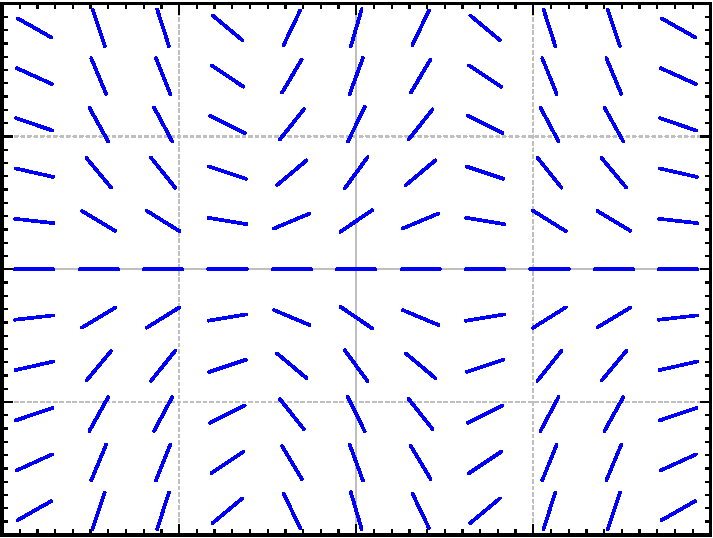
\includegraphics[width=1.75in]{figures/yprimecosxyslope}}
\task
\parbox[c]{1.75in}{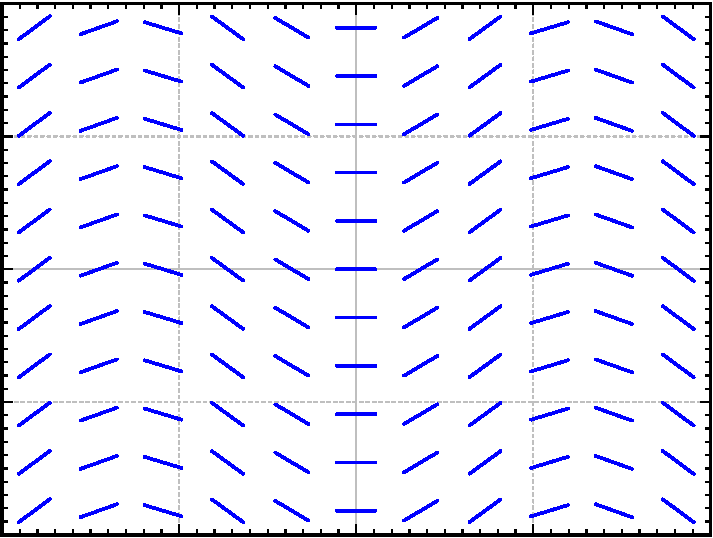
\includegraphics[width=1.75in]{figures/yprimesinxslope}}
\end{tasks}
\end{exercise}
\exsol{%
a) $y'=\cos y$, \quad
b) $y' = y\cos(x)$, \quad
c) $y'=\sin x$. \quad
Justification left to reader.
}

\begin{exercise}
Match equations $y'=y(y-2)$, $y'=y-1$, $y' = y(2-y)$ to slope fields.
Justify.
\begin{tasks}(3)
\task
\parbox[c]{1.75in}{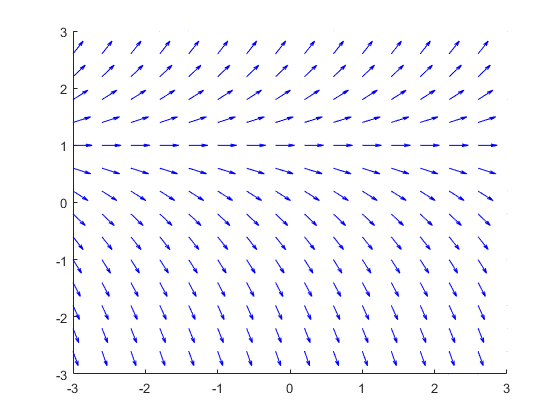
\includegraphics[width=2in]{Images/quivym1}}
\task
\parbox[c]{1.75in}{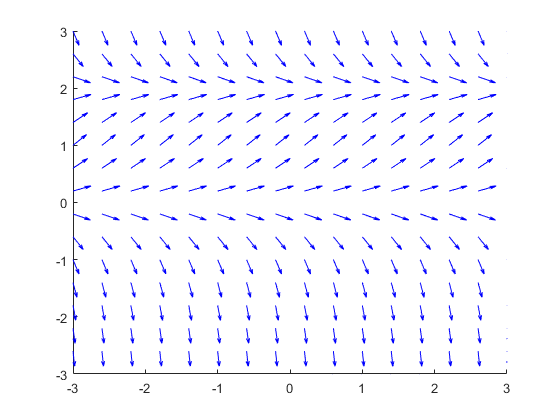
\includegraphics[width=2in]{Images/quivy2my}}
\task
\parbox[c]{1.75in}{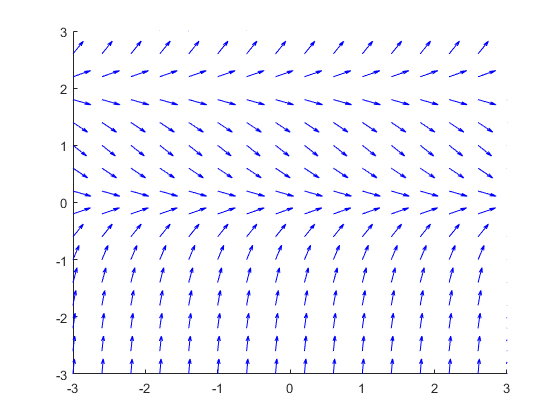
\includegraphics[width=2in]{Images/quivyym2}}
\end{tasks}
\end{exercise}
\comboSol{%
}
{%
a)~$y'=y-1$\quad b)~$y'=y(2-y)$\quad c)~$y'=y(y-2)$
}

\begin{exercise}
Match equations $y'=t(y^2 + 1)$, $y'=t(y^2 - 1)$, $y' = t^2(y^2 - 1)$ to slope fields.
Justify.
\begin{tasks}(3)
\task
\parbox[c]{1.75in}{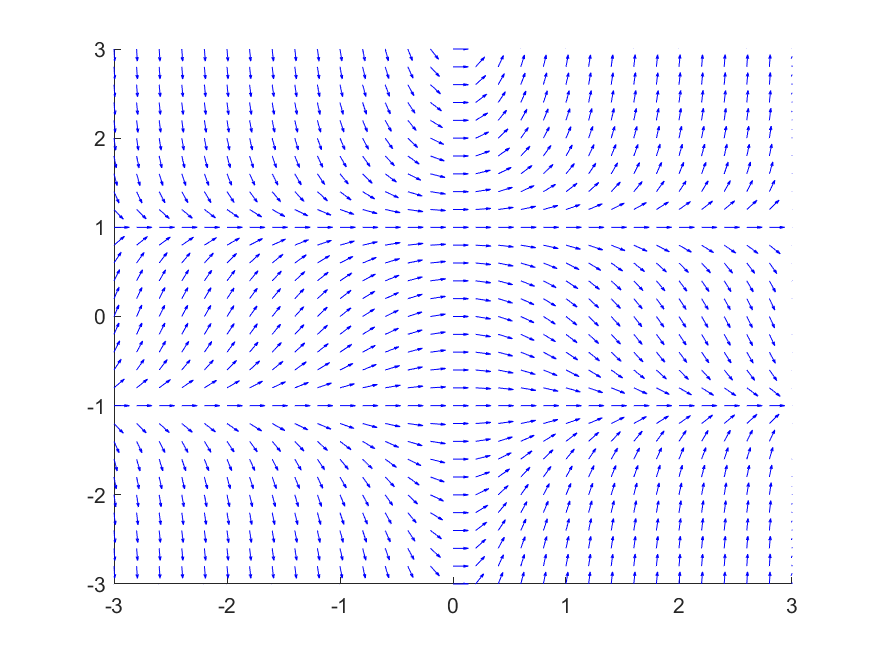
\includegraphics[width=2in]{Images/yprimetysqm1slope}}
\task
\parbox[c]{1.75in}{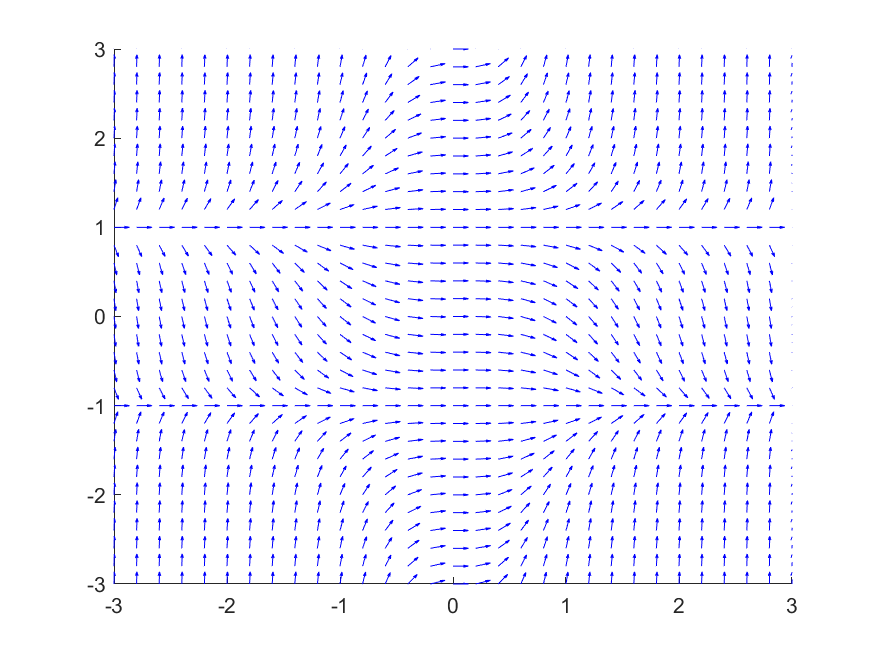
\includegraphics[width=2in]{Images/yprimetsqysqm1slope}}
\task
\parbox[c]{1.75in}{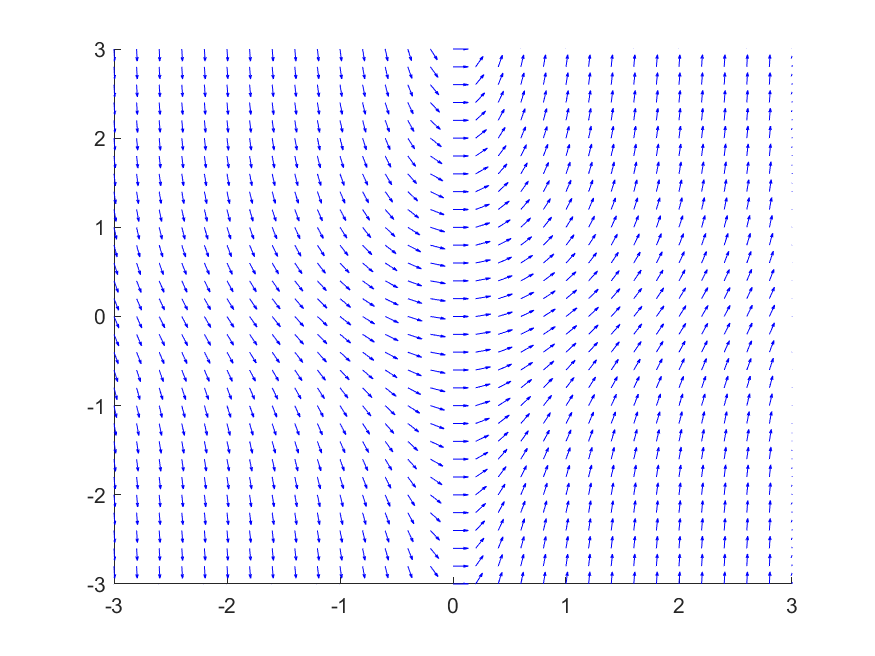
\includegraphics[width=2in]{Images/yprimetysqp1slope}}
\end{tasks}
\end{exercise}
\comboSol{%
}
{%
a)~$y'=t(y^2 -1)$ \quad b)~$y'=t^2(y^2 - 1)$ \quad c)~$y'=t(y^2 + 1)$
}

\begin{exercise}\label{ex:3myyp2}
The slope field for the differential equation $y' = (3-y)(y+2)$ is below. 
If we find the solution to this differential equation with initial condition, $y(0) = 1$, what will happen to the solution as $t \rightarrow \infty$? Use the slope field and your knowledge of the equation to determine the long-time behavior of this solution.
\end{exercise}
\comboSol{%
}
{%
Tends to 3
}

\begin{exercise}\label{ex:tm2yp4ym3}
The slope field for the differential equation $y' = (t-2)(y+4)(y-3)$ is below. 
If we find the solution to this differential equation with initial condition, $y(0) = 1$, what will happen to the solution as $t \rightarrow \infty$? Use the slope field and your knowledge of the equation to determine the long-time behavior of this solution.
\end{exercise}
\comboSol{%
}
{%
Tends to -4
}

\begin{exercise}\label{ex:yp1yp4}
The slope field for the differential equation $y' = (y+1)(y+4)$ is below. 
If we find the solution to this differential equation with initial condition, $y(0) = 1$, what will happen to the solution as $t \rightarrow \infty$? Use the slope field and your knowledge of the equation to determine the long-time behavior of this solution.
\end{exercise}
\comboSol{%
}
{%
Goes to $\infty$. Will not exist for all positive $t$ values.
}

\begin{minipage}{0.32\textwidth}
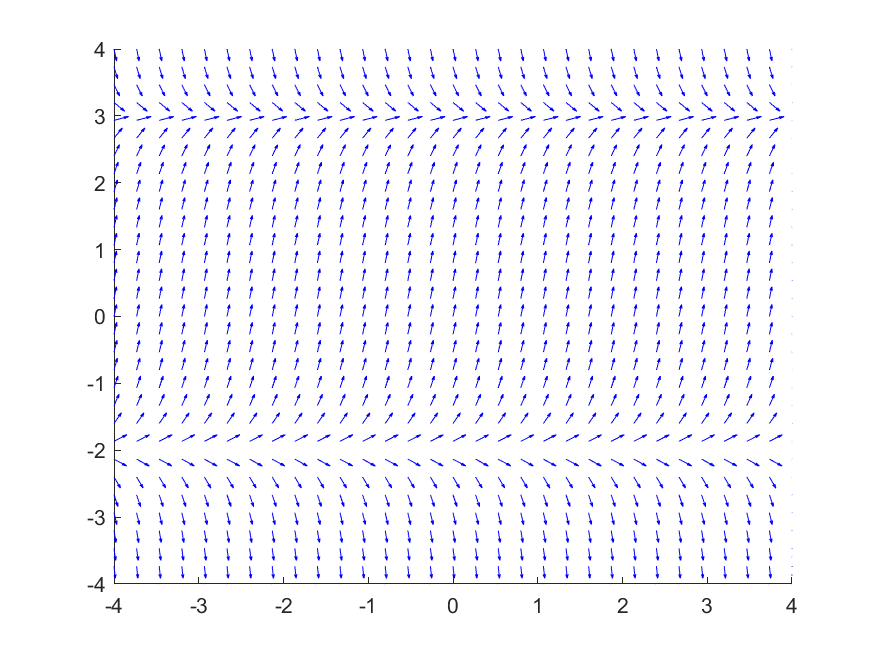
\includegraphics[width=\textwidth]{Images/yprime3myyp2slope}
\captionof{figure}{\exerciseref{ex:3myyp2}}
\end{minipage}%
\begin{minipage}{0.32\textwidth}
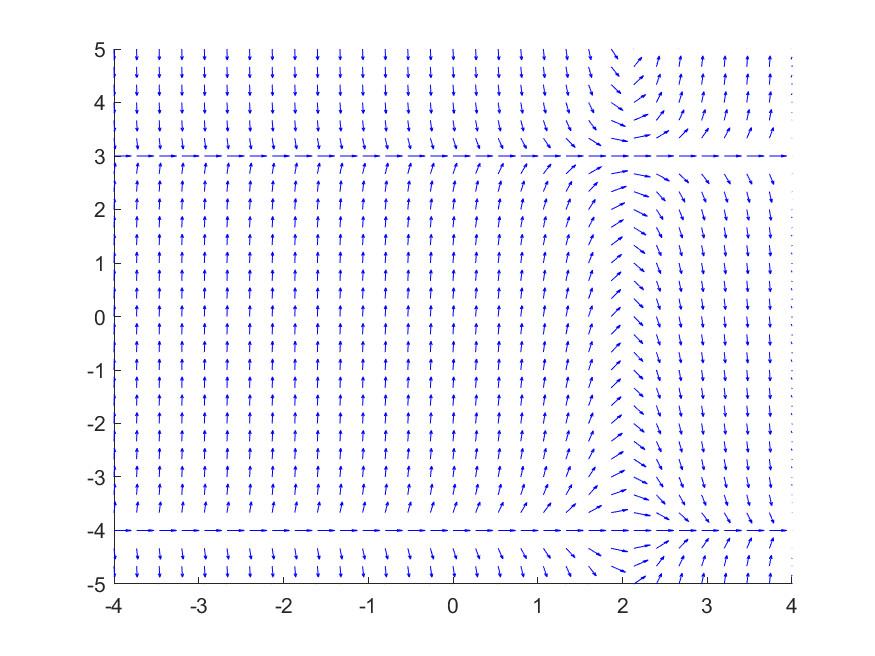
\includegraphics[width=\textwidth]{Images/yprimetm2yp4ym3slope}
\captionof{figure}{\exerciseref{ex:tm2yp4ym3}}
\end{minipage}%
\begin{minipage}{0.32\textwidth}
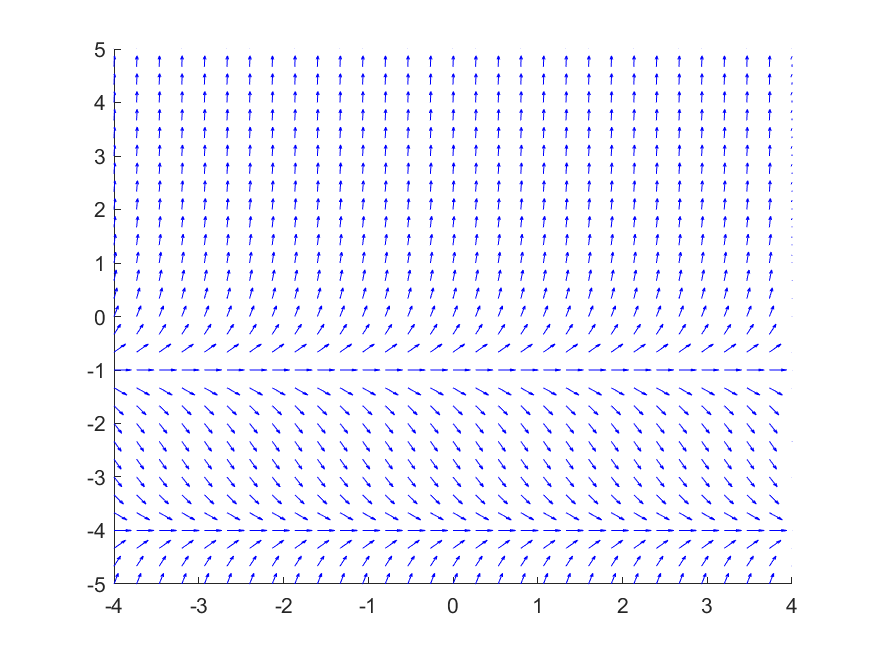
\includegraphics[width=\textwidth]{Images/yprimeyp1yp4slope}
\captionof{figure}{\exerciseref{ex:yp1yp4}}
\end{minipage}

\begin{exercise}[challenging]
Take $y' = f(x,y)$, $y(0) = 0$, where $f(x,y) > 1$
for all $x$ and $y$.  If
the solution exists for all $x$, can you say
what happens to $y(x)$ as $x$ goes to positive infinity?  Explain.
\end{exercise}
\comboSol{%
}
{%
Yes, it will go to $\infty$.
}

\begin{exercise}
Suppose $y' = f(x,y)$.  What will the slope field look like, explain and
sketch an example, if you know the following about $f(x,y)$:
\begin{tasks}(2)
\task $f$ does
not depend on $y$.
\task $f$ does not depend on $x$.
\task $f(t,t) = 0$ for any
number $t$.
\task $f(x,0) = 0$ and $f(x,1) = 1$ for all $x$.
\end{tasks}
\end{exercise}
\comboSol{%
}
{%
a)~Slopes are independent of $y$. On a vertical line, the slopes are all the same. \\
b)~Slopes are independent of $x$. Horizontal invariance. \\
c)~Horizontal tangents along the line $y=x$.\\
d)~Horizontal tangents along the $x$-axis, so $x=0$ is a solution. Slope $1$ along $y=1$. 
}

\begin{exercise}
Describe what each of the following facts about the function $f(x,y)$ tells you about the slope field for the differential equation $y' = f(x,y)$.
\begin{tasks}
\task $f(2,y) = 0$ for all $y$
\task $f(x,-x) = 0$ for all $x$
\task $f(x,x) = 1$ for all $x$
\task $f(x, -1) = 0$ for all $x$
\end{tasks}
\end{exercise}
\comboSol{%
}
{%
a)~Horizontal tangents along $x=2$.\\
b)~Horizontal tangents along the line $y=-x$.\\
c)~Slope one along the line $y=x$. Also $y=x$ is a solution.\\
d)~Horizontal tangents along the line $y=-1$.
}

\setcounter{exercise}{100}

